\documentclass[11pt]{article}

\usepackage{amsmath}
\usepackage{textcomp}
\usepackage[top=0.8in, bottom=0.8in, left=0.8in, right=0.8in]{geometry}
\usepackage{graphicx}
% Add other packages here %

\usepackage[ruled,vlined]{algorithm2e}

% Put your group number and names in the author field %
\title{\bf Excercise 3\\ Implementing a deliberative Agent}
\author{Group \textnumero : 272257, 262609}


% N.B.: The report should not be longer than 3 pages %


\begin{document}
\maketitle

\section{Model Description}
% The problem studied in this report is once again the pickup and delivery problem. This time, our goal is to implement a deliberative agent. This agent establishes a complete plan before doing anything. The plan is supposed to render the best efficiency in terms of cost to deliver the given tasks. Once the plan is established, the agent will act accordingly. If only one agent is present on the tracks, the agent will execute the plan in its entirety and will stop, as nothing has to be done anymore. If two or more agents are present, it can be that one agent disrupt the plan of the other. What happens in that case is that the agent which finds its plan unexecutable will compute one once again with updated informations about the environement when encountering an undoable action (ex: picking up a contract that has already been picked up by an other agent earlier). To establish the plan, we will use research algorithms \emph{BFS} and \emph{A*} on trees. The nodes of the trees will be implemented by the class \emph{State}.% 

\subsection{Intermediate States}
% Describe the state representation %
The states are described by the following attributes:
\begin{itemize}
	\item[$\bullet$] logist.topology.Topology.City \emph{city}, the city the agent is currently in,
	\item[$\bullet$] LinkedList$<$Task$>$ \emph{ctask} (default value = $empty$), that represent the list of tasks the agent has picked up. Note that the elements of the list also have 3 attributes : $pickupCity$ that represents the city the agent can pick up the contract at, $deliveryCity$ that represents the city the agent must deliver the contract at, and $weight$ that represents the weight of the contract,
	\item[$\bullet$] LinkedList$<$Task$>$ \emph{free\_tasks} (default value = $tasks\ present\ in\ the\ environement$), that represents the list of tasks that have not been picked up yet. The elements of the list have the same attributes as in the list mentioned before,
	%\item[$\bullet$] State \emph{parent} (default value = $null$) is the predecessor of the current state. This will be used after the application of the \emph{BFS} and \emph{A*} algorithms to build back the plan from the goal state we find using those algorithms,
	\item[$\bullet$] double \emph{cost} (default value = $0$), the sum of all steps needed to get to this state, 
	%\item[$\bullet$] Act \emph{act} (default value = $START$), represents the action taken at the given state. This value can vary between \emph{START}, \emph{PICKUP}, \emph{MOVE} and \emph{DELIVER}. The meaning of these actions will be given in a section below.
	%\item[$\bullet$] int \emph{depth} (default value = $0$), that represents the depth of the nodes in the tree,
	%\item[$\bullet$] Boolean \emph{heuristic}, that represents the method used by the search algorithm. If $heuristic=true$, then the \emph{A*} algorithm is used. Otherwise the \emph{BFS} algorithm is used,
	\item[$\bullet$] a method long $cweight()$, that returns the sum of the weight of the current tasks.
	%\item[$\bullet$] a method Stack$<$State$>$ $succ(\mathrm{Topology}\ topology,\mathrm{int}\ capacity) $, that returns all the possbile children of the current node, where the parameter is the maximal capacity of an agent.
\end{itemize}

%Note that we also have a constant called $capacity$ stored in the $Deliberative$ class (see below) that represents the maximal weight that can be loaded into an agent. This constant will be passed in the successor function each time it is called.

\subsection{Goal State}
% Describe the goal state %
A goal state is defines as a state at with all tasks have been picked up and delivered. Translated , this gives the condition $ctask.size() == 0\ \&\&\ free\_tasks.size() == 0$. 

\subsection{Actions}
% Describe the possible actions/transitions in your model %
%The agent has 4 different possibilities of action. An action is implemented by the $act$ variable in the $State$ class, it defines what the children of a node can be, i.e. the result of the successor function. We provide a clearer explanation. Suppose we have a state $state$. %We will only give the attributes that change, the rest is assumed to be directly inherited from the parent except for the $parent$ attribute that is set to $state$. Note that all combination of mentioned cases can happen and thus we generate a child node for each individual possibility if not mentioned otherwise.\\
% \begin{itemize}
%	\item[$\bullet$] \underline{If $state.act=START$:} Then we can have 
%		\begin{align*}
%					 PICKUP &,\ \mathrm{if}\ state.city\in\{task.pickupCity\ |\ task\in state.free\_tasks\},\\
%					 MOVE &,\ \mathrm{in\ any\ case}.
%				       \end{cases}
%		\end{align*}
%If $state.act = START$, then we are at the very beginning of the simulation. We then have that $state.succ.capicity$ is the list of states that have either $PICKUP$, if a task can be picked at the given city, $MOVE$.\\
%If $state.act = PICKUP$, then we have that the children have their $ctask$ attribute set to $state.ctask.add(task)$, their $free\_tasks$ attribute to $state.free\_tasks.remove(task)$, where $task$ is the task picked up at that moment, and their $act$ attribute to either $PICKUP$, $MOVE$ or $DELIVER$ if possible.\\
	%\item[$\bullet$] \underline{If $state.act=PICKUP$:} Note that it means that we have that there exists $task\in state.free\_tasks$ such that $task.pickupCity=state.city$ and $capacity-state.cweight()\geq task.weight$. Then we can have 
		%\begin{align*}
			%s'.ctask =& s.ctask.add(task),\\
			%s'.free\_tasks =& s.free\_tasks.remove(task),\\
			%s'.act =& \begin{cases}
			%			PICKUP &,\ \mathrm{if}\ state.city\in\{task.pickupCity\ |\ task'\in state.free\_tasks.remove(task)\\ & \&\&\ capacity-state.cweight() - task.weight \geq task'.weight\},\\
					%	MOVE &,\ \mathrm{in\ any\ case},\\
				%		DELIVER &,\ \mathrm{if}\ state.city\in\{task.deliveryCity\ |\ task\in state.ctask\}.
					%\end{cases}
		%\end{align*}
%If $state.act = DELIVER$, then we have that the children must have their $ctask$ attribute set to $state.ctask.remover(task)$, where $task$ is the task being deliverd, and their $act$ attribute can either be set to $PICKUP, MOVE$ or $DELIVER$ according to the courant environnement.\\
	%\item[$\bullet$] \underline{If $state.act=DELIVER$:} Note that this means that we have a task $task\in state.ctask$ such that $task.deliveryCity = state.city$. Then we can have
		%\begin{align*}
			%s'.ctask =& state.ctask.remove(task),\\
			%s'.act =& \begin{cases}
					%	PICKUP &,\ \mathrm{if}\ state.city\in\{task'.pickupCity\ |\  task'\in state.free\_tasks\\
						%& \&\&\ capacity-state.cweight() + task.weight \geq task'.weight\},\\
						%MOVE &,\ \mathrm{in\ any\ case},\\
						%DELIVER &,\ \mathrm{if}\ state.city\in\{task.'pickupCity\ |\ task'\in state.ctask.remove(task)\}.
			%		\end{cases}
		%\end{align*}
		
%If $state.act = MOVE$, then we that the children must have theire $city$ attribute set to some $city'$ in the neighbourhood of $state.city$ and their $cost$ attribute must be set to $state.cost+state,city.distanceTo(city')$. Their $act$ attribute can be either set at $PICKUP, MOVE$ or $DELIVER$ according to the courant environnement.	
	%\item[$\bullet$] \underline{If $state.act=MOVE$}:  Then for each $city'$ such that $state.city.isNeighbour(city')$, we can have 
		%\begin{align*}
			%s'.city =& city',\\
			%s'.cost =& state.cost+state.city.distanceTo(city'),\\
			%s'.act =& \begin{cases}
					%	PICKUP &,\ \mathrm{if}\ city'\in\{task.pickupCity\ |\ task\in state.free\_tasks\\
						%		& \&\&\ capacity -state.cweight()\geq task.weight\},\\
						%MOVE &,\ \mathrm{in\ any\  case},\\
						%DELIVER  &, \mathrm{if}\ city'\in\{task.deliveryCity\ |\ task\in state.ctask\}.
					%\end{cases}
		%\end{align*}
%\end{itemize}

We distinguish three types of steps (that can be though of as an a edge between node-states in the graph). \textbf{Move-edges} that represent the physical movement of the agent (a change to a \emph{neighbor} city) and a have a cost equal to the distance between the two cities, \textbf{Pickup-edges} that represent the picking up of a task (and therefore can only happen in a city where a task is available) and have no cost (but has an influence on the carried weight of the agent, its remaining-capacity, and available tasks) and \textbf{deliver-edges} that represent the act of delivering a task, those have no cost but have an influence of the carried weight of the agent and its remaining-capacity. \\

Note that this generate a lot of nodes at each iteration. In practice, in the $A^*$  and $BFS$, we always choose the \textbf{deliver-edges} when it is possible. This reduces consequently the number of possible states at certain times. It seems also intuitive to deliver a task when said task has been picked up and the agent happens to pass through its delivery city. Not doing so would automatically be non-optimal. That is why this restriction actually helps us in the plan making process.

\section{Implementation}
We implemented those two algorithms in the $Deliberative$ class. We suppose that we begin at the city $city$.
\subsection{BFS and A*}
% Details of the BFS implementation %
\begin{algorithm}[H]
	\SetAlgoLined
%	\Kwresult{A state $s$ goal with minimal cost for this property}
	initialization: Set $Q$ a queue of $State$ objects with one element $state$ at default values with\\  
	\ \ \ \ \ \ \ \ \ \ \ \ \ \ \ \ \ \ \ $state.city = city$ and $state.heuristic = true$ if $A^*$ and $false$ if $BFS$ and set $C$ to\\ \ \ \ \ \ \ \ \ \ \ \ \ \ \ \ \ \ \ \ be an empty queue.\\
	$s\leftarrow nil$\\
	\While{$Q.size()\geq1$ and $s$ is not a goal state}{
		$s\leftarrow Q.pop()$\\
		\If{$s.goal()$}{
			\Return{$s$}
		}
		\If{$s.rajoute(C)$}{
			$Q\leftarrow Q + s.succ(topology, capacity)$\\
			$Q\leftarrow Q+succ(s)$\\
			\If{Algorithm is $A^*$}{
				$Q.sortBy(f)$
			}
			\If{Algorithm isn't $A^*$}{
				$Q.sortBy((s'\mapsto s'.cost))$
			} 
		}
	}
	\Return{$nil$}
	\caption{$BFS$ and $A^*$}
\end{algorithm}
where the functions $s.rajoute(C)$ takes a queue  $f(s) = s.cost + s.heuristic()$. %This heuristic function represents an estimation of the minimal cost of operations needed to get to a goal state. It is described exactly in the following section.

\subsection{Heuristic Function}
% Details of the heuristic functions: main idea, optimality, admissibility %
The heuristic function is given by 
	\begin{align*}
		s.heuristic() & = \begin{cases}	
							max \{s.city.distanceTo(task.pickupCity)+\\ \ \ \ \ \ +task.pickupCity.distanceTo(task.deliveryCity)\},\\
							max  \{s.city.distanceTo(task.deliverCity)\}.
						\end{cases}
	\end{align*}
where the maximum is taken on the set $$\{task\in s.free\_tasks\ \}$$ in the first case when it is not empty, and on $$\{task\in s.ctask\}.$$ in the second case, when the first set is empty. We claim that such an heuristic is optimal for the $A^*$ algorithm. Indeed, one easily sees that in order to get to a goal state, one needs at least to pick and deliver the remaining tasks that were not picked up before, especially the farthest one. This is the exactly the value $s.heuristic$ takes in the first case. In the second one, assuming that all the tasks were picked up, one still needs to deliver each tasks that has yet to be deliverde. In particular the farthest one. This corresponds to taking this maximum in the second case. \\
As the seen in the course this allows us to say that $A^*$ does find the optimal plan. This heuristic function was inspired by trying to force the agent to take a maximum of tasks and the deliver them.

\section{Results}

\begin{figure}[h!]
	\centering
	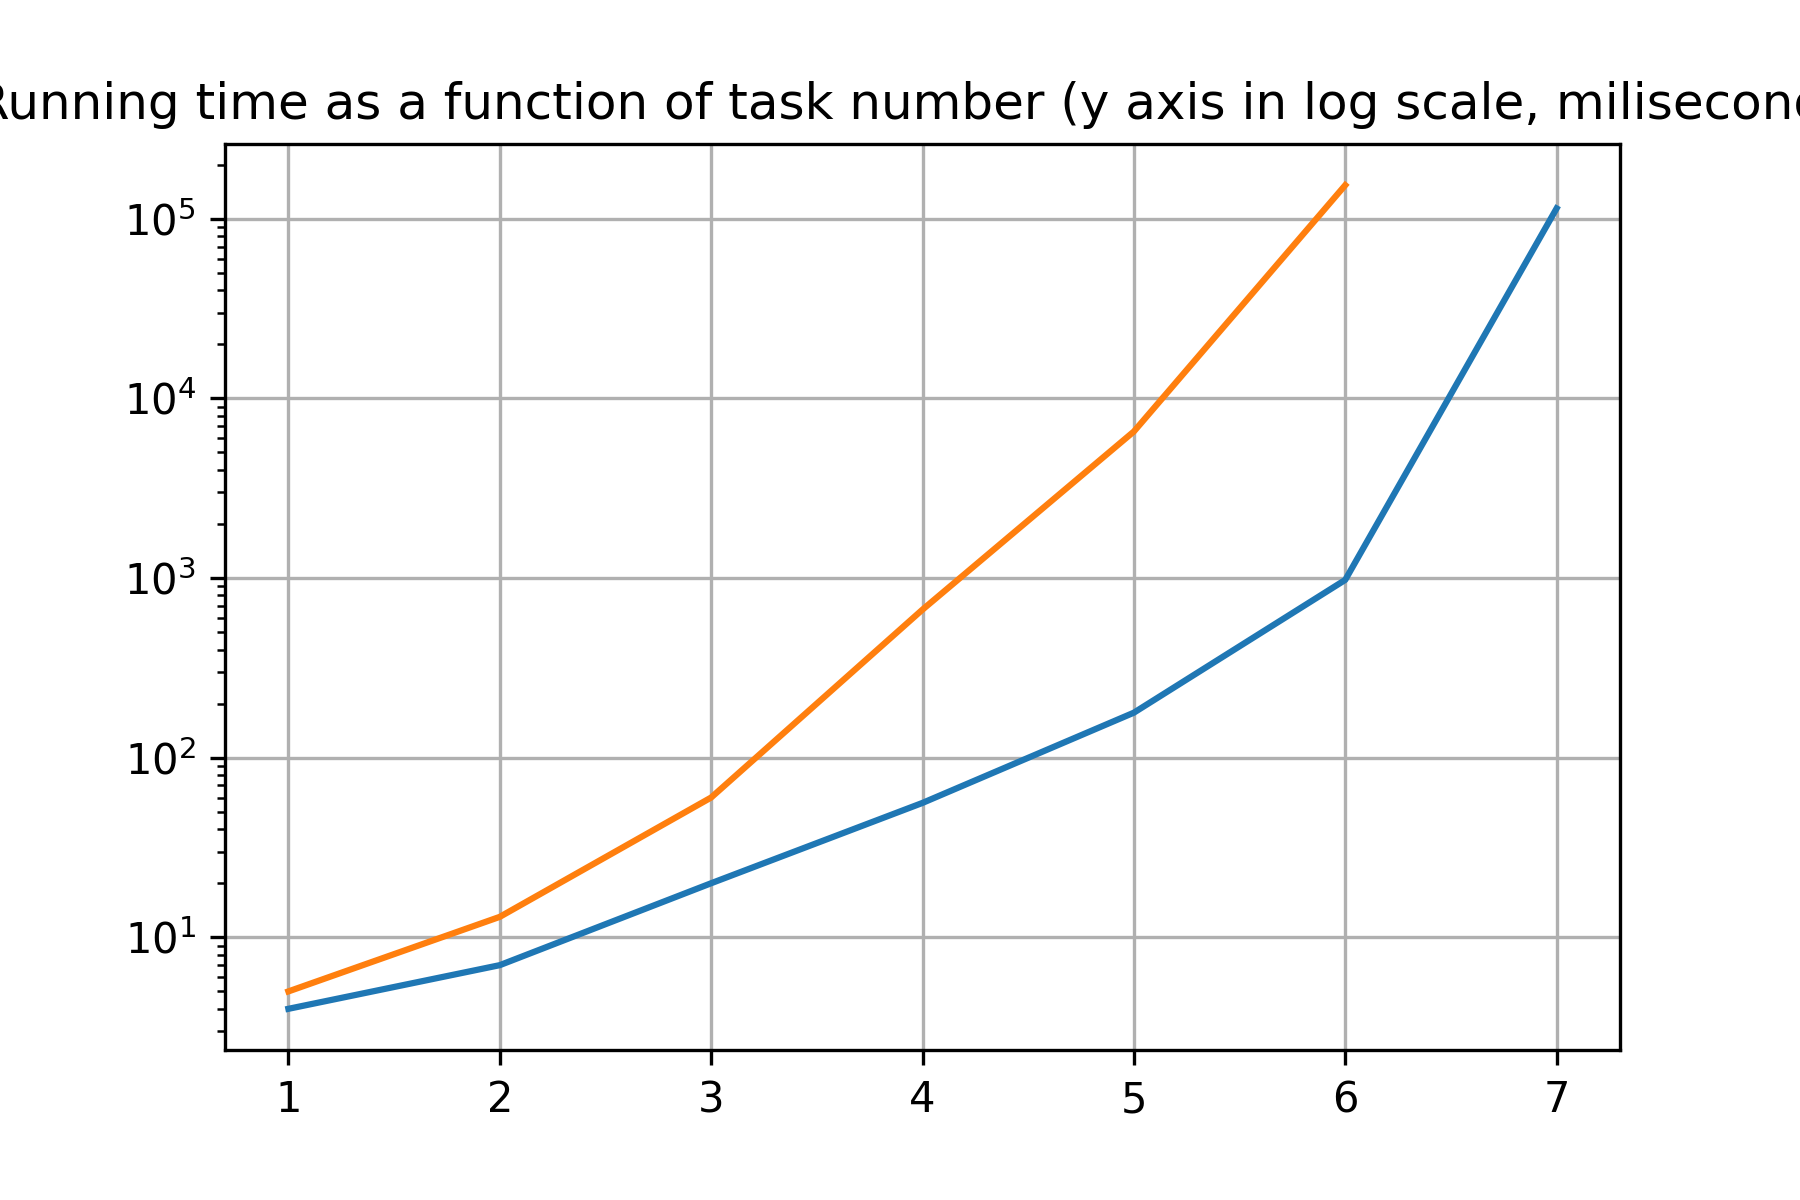
\includegraphics[width=0.4\textwidth]{runningTime.png}
	\caption{Compared running times of $BFS$ (orange) and $A^*$ (blue) (y axis in log scale, milliseconds).}
  \end{figure}

\subsection{Experiment 1: BFS and A* Comparison}
% Compare the two algorithms in terms of: optimality, efficiency, limitations %
% Report the number of tasks for which you can build a plan in less than one minute %

\subsubsection{Setting}
We run simulations for $BFS$ and $A^*$ agents, with seed $2342356$ on the "Switzerland" map and raise the task number until running time $T(n_{tasks})$ until $T(n_{tasks})\geq 1min$.

\subsubsection{Observations}

We observe that $BFS$ grows clearly faster than $A^*$ that we are able to optimize for $5$ tasks with $BFS$ and $6$ tasks with $A^*$ in under a minute. We also observe that the running times grows faster than $O(e^n)$ for both algorithms (see Figure 1).
% Describe the experimental results and the conclusions you inferred from these results %


\subsection{Experiment 2: Multi-agent Experiments}
% Observations in multi-agent experiments %



\subsubsection{Setting}
We run simulations (again with seed $2342356$ on the "Switzerland" map) with a varying number (1 to 3) of $A^*$ agents to observe their interactions when optimizing on the same state-space. In order to have some point of reference we run the same experiment with \emph{naive} agents as well.

\subsubsection{Observations}
\begin{center}
	\includegraphics[width=0.8\textwidth]{tableau.png}
\end{center}
We observe that if we optimize for distance, a single $A^*$ agent is more efficient than any other tested scenario (here we consider total distance traveled by all the agents in the scenario). Adding other $A^*$ agents reduces performance. This cannot be said if we optimize over time, then adding more agents is actually beneficial (but we observe that the more agents we add the less improvement we see).
% Describe the experimental results and the conclusions you inferred from these results %


\end{document}